\documentclass[letterpaper]{article} % DO NOT CHANGE THIS
\usepackage[submission]{aaai2027}  % DO NOT CHANGE THIS
% The serif, sans-serif, and monospaced fonts are loaded automatically by
% aaai2027.sty (newtxtext, helvet, courier). DO NOT add \usepackage{times},
% \usepackage{helvet}, \usepackage{courier}, or any other font package.
\usepackage[hyphens]{url}  % DO NOT CHANGE THIS
\usepackage{graphicx} % DO NOT CHANGE THIS
\urlstyle{rm} % DO NOT CHANGE THIS
\def\UrlFont{\rm}  % DO NOT CHANGE THIS
\usepackage{natbib}  % DO NOT CHANGE THIS AND DO NOT ADD ANY OPTIONS TO IT
\usepackage{caption} % DO NOT CHANGE THIS AND DO NOT ADD ANY OPTIONS TO IT
\frenchspacing  % DO NOT CHANGE THIS

\usepackage{amsmath,amssymb}
\usepackage{booktabs}
\newcommand{\model}{Qwen-Image-Edit-2511}
\newcommand{\eg}{\emph{e.g.}}
\newcommand{\ie}{\emph{i.e.}}

% Keep the \pdfinfo as shown here. There's no need
% for you to add the /Title and /Author tags.
\pdfinfo{
/TemplateVersion (2027.1)
}

\setcounter{secnumdepth}{0} % AAAI: unnumbered sections by default

\title{Predictable Early, Translated Late: A Layer--Time Lens for Diffusion Image Editors}
\author{
    Anonymous Submission
}
\affiliations{
    %
}

\begin{document}

\maketitle

\begin{abstract}
Between reading an edit instruction and painting pixels, what does a
diffusion-transformer (DiT) image editor represent? We build a layer--time
lens that decodes intermediate residuals through the model's frozen output
head and pairs readouts with linear probes and activation interventions
(ablation, transplant, steering). On fixed underspecified recoloring
prompts, the \emph{realized} outcome is predictable from early layers
while the frozen head still reads noise (car color: $0.667$ balanced
accuracy vs.\ chance $0.333$, $p{=}0.002$). That target-image code is
\emph{translated late} into the velocity field near layers 52--54 of 60:
the crossover midpoint changes by under one layer between tested timesteps,
although its width is timestep-dependent. The boundary replicates in an
independent fine-tune and a four-step distilled checkpoint of the same
Qwen lineage; held-out early best-of-five selection validates the readout
on a second architecture. Transplant establishes sufficiency; in the tested
recolor setting, steering shows writable hue requires a spatial carrier. Truncating
classifier-free guidance after step two saves 45\% of forward passes on
tested edits.
\end{abstract}

% BEGIN expanded input: aaai_draft/00_intro
% ===== AAAI-27 spine draft: Introduction (~0.9 col-page target) =====
\section{Introduction}\label{sec:intro}

Between reading ``turn the car red'' and painting it, what does a
diffusion image editor actually do? The mechanics of diffusion suggest
a gradual-development story, each of sixty blocks and twenty denoising
steps contributing its small share -- but this paper measures that
story and finds it wrong. In the model we study, the realized edit is
\emph{predictable early} from an internal target-image code, and only
\emph{translated late}, in the last few blocks, into the flow field that does
the painting.

Prior work provides partial readouts of generative internals. The logit and
tuned lenses project transformer residuals through a final or learned output
map~\citep{nostalgebraist2020logitlens,belrose2023tuned}. In diffusion,
Diffusion Lens interprets text-encoder states; DiffLens and ICM probe or steer
denoiser features; and DreamReader and sparse autoencoders provide broader
extraction and feature-analysis tools
~\citep{toker2024diffusionlens,shi2025difflens,zaleska2026icm,prakash2026dreamreader,surkov2025sae}.
Linear-representation work motivates a probe-readable basis, while multimodal
reasoners externalize visual thoughts as sketches or whiteboards
~\citep{park2024linear,hu2024sketchpad,menon2024whiteboard,wu2024vot,li2025mvot};
we instead test for an unrendered internal image, complementing the broader
thinking-with-images taxonomy~\citep{su2025thinkingsurvey}.
Recent work also detects early cross-seed convergence, predicts final quality
from early activations, or allocates adaptive image-editing budgets
~\citep{kwon2026lockin,guo2026probeselect,qu2026adecot}. None jointly decodes
an instruction-based DiT's image stream across both transformer depth and
denoising time while separating explicit-prompt readability from the realized
outcome under a fixed prompt.

A second line studies how to produce edits or intervene on hidden states.
Modern editors build on diffusion, latent/flow formulations, and guidance
~\citep{ho2020ddpm,song2021ddim,rombach2022ldm,lipman2023flowmatching,liu2023rectifiedflow,ho2022cfg}.
InstructPix2Pix and Prompt-to-Prompt learn or manipulate diffusion editing
controls~\citep{brooks2023instructpix2pix,hertz2023prompttoprompt}; ROME and
activation-patching practice transfer hidden states, while activation
engineering adds steering directions
~\citep{meng2022rome,heimersheim2024activation,turner2023actadd}. Concept
Lancet already uses representation transplant for diffusion editing
~\citep{luo2025colan}. Recent analyses further show that detectable diffusion
features can fail under steering and that multi-mediator patching can hide
interaction effects~\citep{cassano2026look,vaidyanathan2026curse}. We therefore
use transplant only as a sufficiency test and steering only as a bounded
writability test, not as a standalone editing method or a necessity proof.

We build a layer--time lens for a production DiT editor,
\model{} (60 blocks)~\citep{peebles2023dit,qwen2025image}, by decoding intermediate residual streams through
the model's own frozen output head, and -- crucially -- pair passive
readings with linear probes and controlled activation
interventions (ablation, transplant, steering) that test what those
activations can install or write.

Naively porting the logit-lens recipe reproduces the familiar mid-stack
``nothing happens yet'' appearance -- and that appearance is itself
misleading. With source and an underspecified recoloring instruction
fixed across 48 seeds, a generation-level probe predicts the color
ultimately chosen from layer 6, where the frozen head still reads noise.
The outcome is held in a basis the head cannot parse until a narrow band
near the top translates it into the velocity field that paints the result.

The main contributions of this work are as follows:
\begin{itemize}
\item \textbf{An instrument.} A layer--time instrument for a DiT image
editor, combining a training-free frozen-head lens with tuned and
differential variants,
paired with linear probes and three intervention primitives (ablate,
transplant, steer) with stated write semantics, under a
falsification-first protocol -- pre-registered predictions, per-image
visual verdicts, and bit-exact gates.
\item \textbf{A mechanism: the editor thinks with an internal image.}
The realized edit is predictable early under a fixed underspecified
instruction, carried as a target-image code, and translated into the
velocity code near layers 52--54. Across the two densely measured
timesteps, the crossover midpoint differs by under one layer while its
width varies from one to four layers; the boundary also replicates in a
same-lineage fine-tune and a 4-step distillation. Transplant establishes
sufficiency; in the tested recolor setting, steering and a rank ladder show
that readable attributes require a spatial carrier and a
variable-dependent write subspace.
\item \textbf{Validation and a lever.} Held-out early best-of-five selection
validates the readout on Qwen and an independent architecture, with about
68\% measured compute reduction. Separately, truncating classifier-free
guidance after step 2 saves 45\% of forward passes across tested edit
families; dropping CFG entirely produces failures consistent with a
non-redundant role in scope resolution rather than outcome selection.
\end{itemize}
This is exploratory, single-model-family work; every verdict was made
on the images themselves, and we are explicit about where the lens is
unreliable.
% END expanded input: aaai_draft/00_intro

\begin{figure}[t]
  \centering
  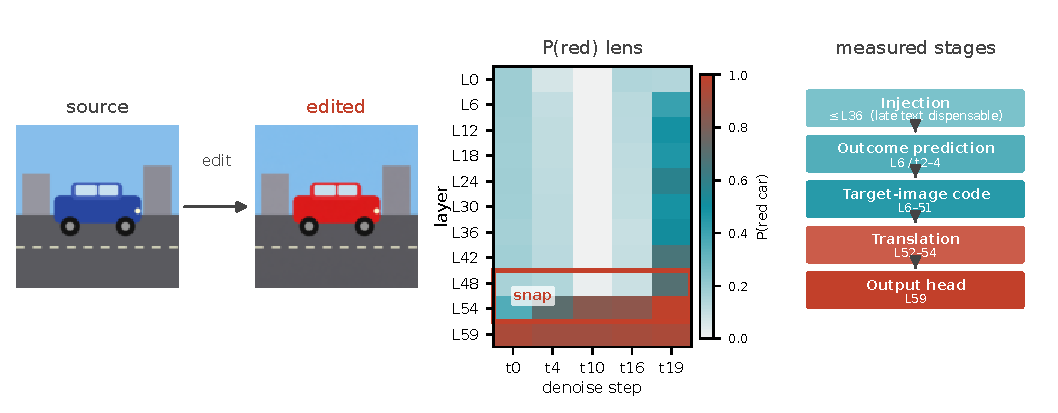
\includegraphics[width=\columnwidth]{figs/fig1_teaser/fig1_teaser.pdf}
  \caption{\textbf{Predictable early, translated late.} \textbf{A}: source
  and realized edit. \textbf{B}: frozen-head $P(\text{red car})$ across
  layer and step; the outcome is probe-readable at L6, but translation
  into the head-readable velocity convention occurs at L52--54.
  \textbf{C}: the five measured stages used throughout the paper.}
  \label{fig:teaser}
\end{figure}

\begin{figure*}[t]
	\centering
	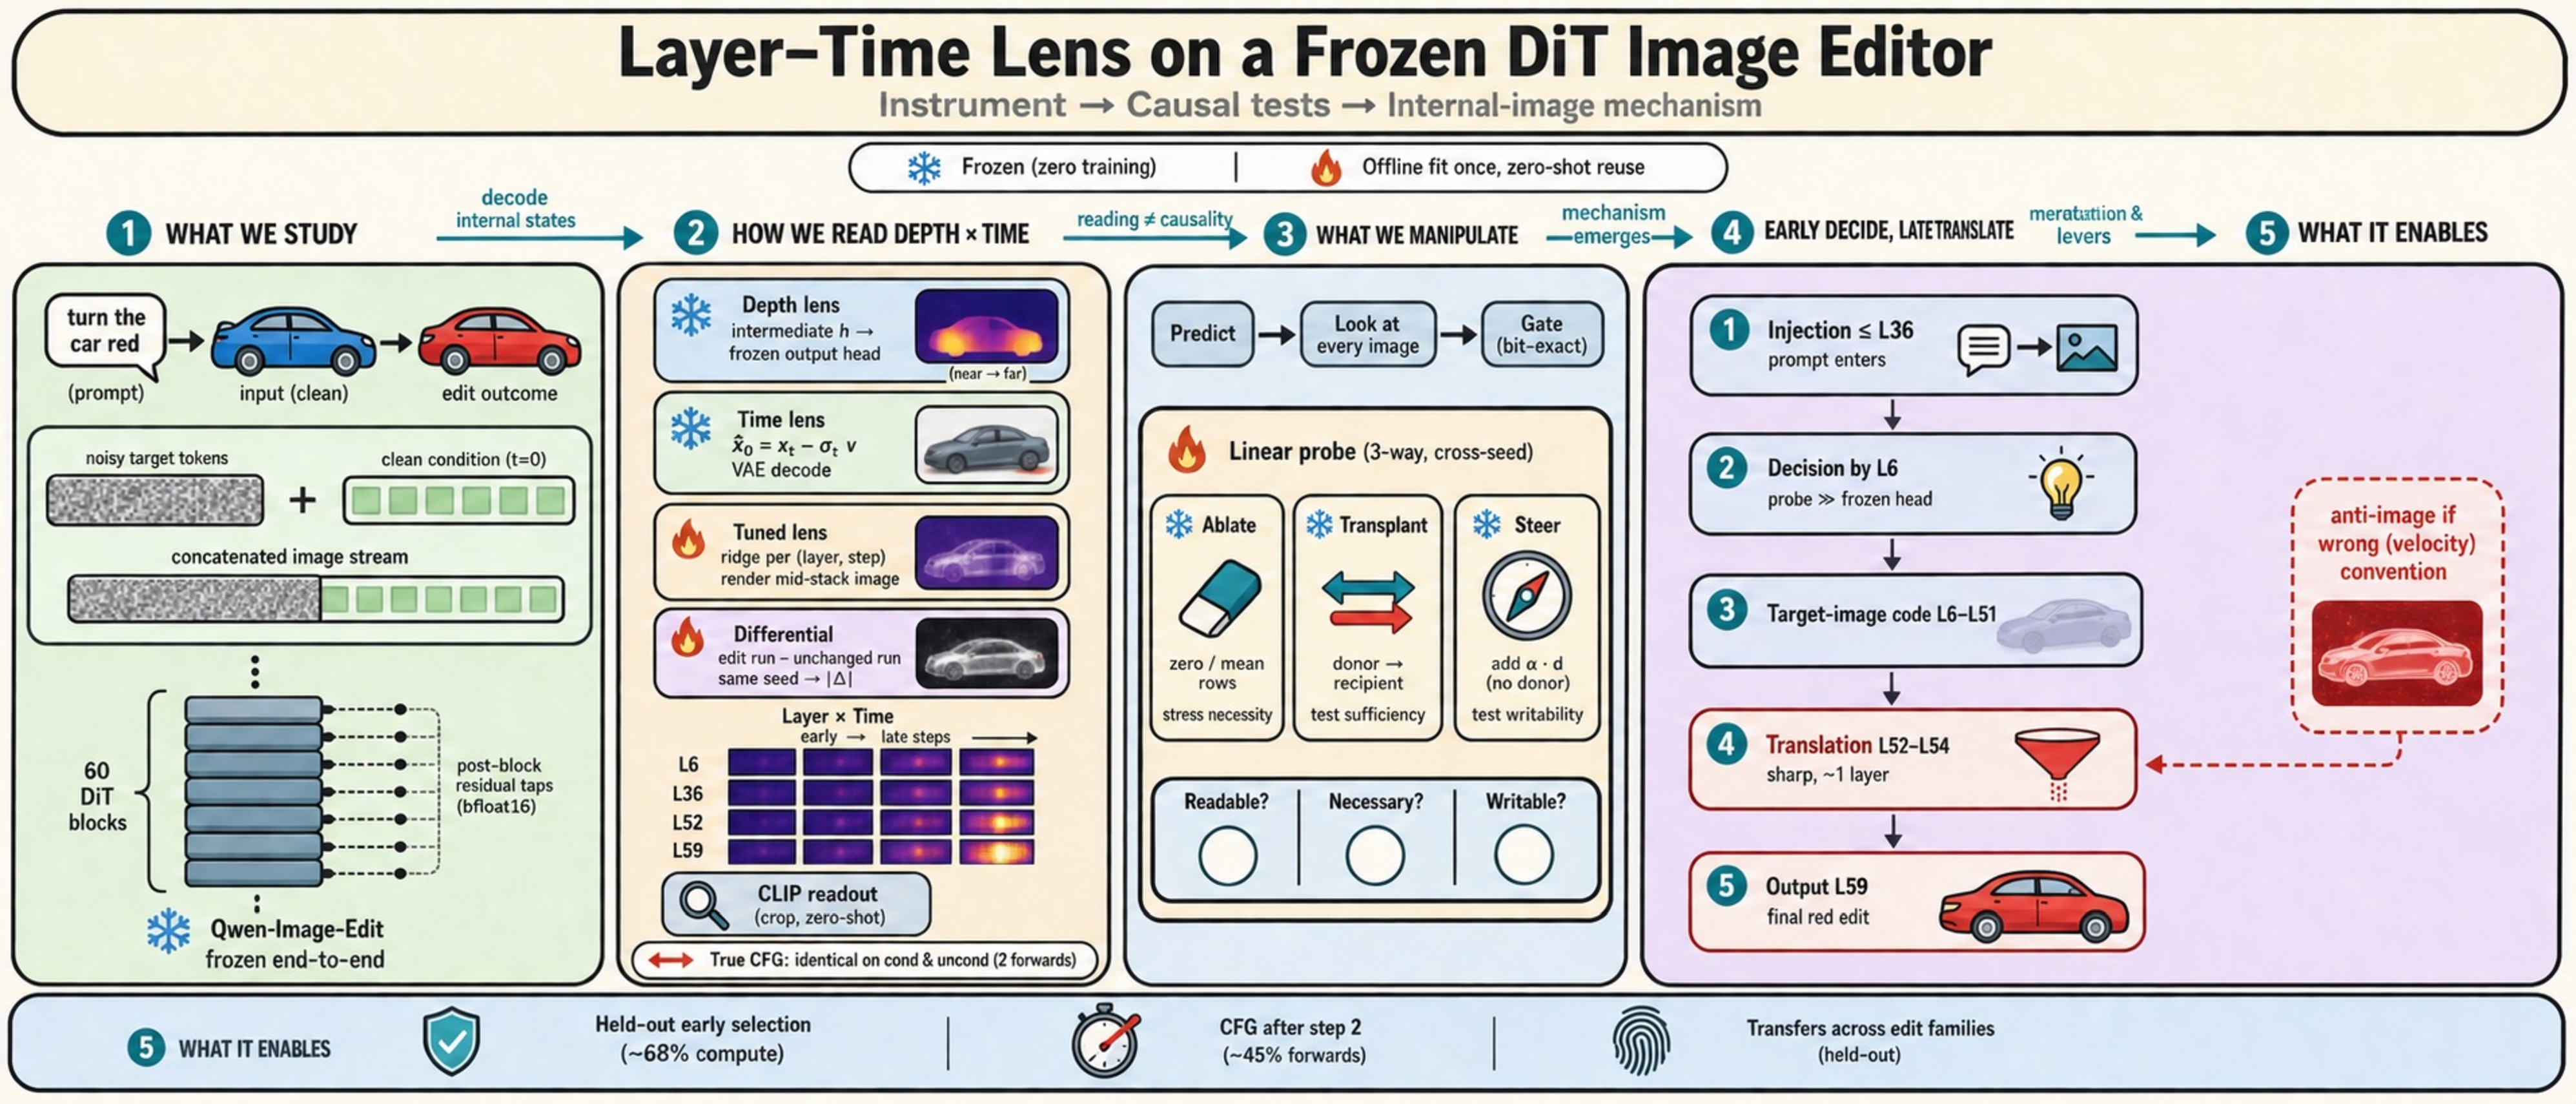
\includegraphics[width=0.95\textwidth]{figs/fig2_method/fig2_method.pdf}
	\caption{\textbf{Framework overview.} Frozen \model{} on a concatenated
		noisy-target / clean-condition image stream with post-block residual
		hooks (\texttt{bfloat16}). \emph{Read}: depth, time, tuned, and
		differential lenses decode previews, then crop-level CLIP scoring on
		matched true-CFG passes. \emph{Test}: linear probes plus ablate,
		transplant, and steer interventions under predict--look--gate protocol.
		\emph{Mechanism} (schematic): early decision and target-image code,
		late L52--L54 translation into the velocity field; bottom: held-out
		validation and training-free levers discussed in text.}
	\label{fig:method}
\end{figure*}

% BEGIN expanded input: aaai_draft/10_method
% ===== AAAI-27 spine draft: Method (~1.3 col-page target) =====
\section{Proposed Method: A Layer--Time Lens and Intervention Probes}\label{sec:method}

Figure~\ref{fig:method} summarizes the full pipeline; here we specify each
component. We study \model{}, a 60-block DiT editor whose image stream
concatenates noisy target tokens with always-clean condition tokens. All
quantities below are read from the
\emph{post-block residual} of selected blocks via forward hooks,
captured in the model's native \texttt{bfloat16}: image-stream
activations reach absmax ${\sim}3{\times}10^{9}$ even at layer 0, so a cast
to \texttt{float16} silently overflows most elements to \texttt{inf}
(bf16 capture is a lossless copy, not a downcast).

\paragraph{Notation and layer--time readout.}
Let $h_{\ell,t}^{(i)}\!\in\!\mathbb{R}^{d}$ denote the post-block residual
after block $\ell\!\in\!\{0,\ldots,59\}$ at denoising step $t$, for
image-stream row $i$ (target patch, condition patch, or a hooked subset);
$h^{\mathrm{tar}}_{\ell,t}$ stacks the target-patch rows used for all
image-space readouts below (condition rows are captured only for explicitly
stated controls). A lens operator
$\mathcal{L}_{\ell,t}:\mathbb{R}^{n\times d}\!\to\!\mathbb{R}^{n\times64}$
maps these residuals to a target-grid velocity estimate $\tilde v_{\ell,t}$.
Logit- and Jacobian-style lenses in language models align internal states
with output units along depth and token position; a DiT patch has no
vocabulary, so we define a \emph{layer--time lens} as a map from
$(\ell,t)$ to an image and then a score on a fixed grid:
\begin{equation}
  I_{\ell,t}
  = \mathcal{V}\!\left(\Pi_t\!\left(
  \mathcal{L}_{\ell,t}(h^{\mathrm{tar}}_{\ell,t})\right)\right),
  \qquad
  \Pi_t(\tilde v)=x_t-\sigma_t\tilde v,
  \label{eq:lens-grid}
\end{equation}
where $\mathcal{V}$ is the frozen VAE decoder. We score a fixed edit-region
crop of $I_{\ell,t}$ with CLIP ViT-L/14~\citep{radford2021clip}. With
unit-normalized image and prompt-ensembled text embeddings $e_I,e_T$, and
CLIP's learned logit scale $\gamma$, the forced-choice probability over the
reported label bank $\{y_k\}$ is
\begin{equation}
  [\mathcal{M}_{\ell,t}]_k
  \;=\;
  \mathrm{softmax}_k\!\Bigl(
    \gamma\, e_T(y_k)^\top e_I(\mathrm{crop}(I_{\ell,t}))
  \Bigr).
  \label{eq:clip-readout}
\end{equation}
Figures~\ref{fig:teaser} and~\ref{fig:method} instantiate
\eqref{eq:lens-grid}--\eqref{eq:clip-readout}: the image-editor analogue of
lexical alignment grids in logit/Jacobian-lens visualizations, not a full
$\partial \mathbf{y}/\partial h$ (a donor-scalar Jacobian basis is tested in
the supplement and does not coincide with probe or write directions).

\paragraph{Lens operators.}
The \emph{time lens} uses the terminal head output at step $t$:
\begin{equation}
  \hat{x}_0(x_t,t) = x_t - \sigma_t\, v_\theta(x_t,t),
  \label{eq:time-lens}
\end{equation}
decoded through the VAE---what the model currently believes it will output.
The \emph{depth lens} asks the same question at intermediate depth by
re-invoking the model's frozen output head (non-affine
\texttt{AdaLayerNormContinuous} + linear \texttt{proj\_out}, bit-exact
whether invoked at layer 59 or earlier):
\begin{equation}
  v_{\ell,t} = \mathrm{Head}(h^{\mathrm{tar}}_{\ell,t}),
  \qquad
  \hat{x}_{0,\ell,t} = x_t - \sigma_t\, v_{\ell,t},
  \label{eq:depth-lens}
\end{equation}
then $I_{\ell,t}=\mathcal{V}(\hat{x}_{0,\ell,t})$.
Because \texttt{norm\_out} has no learned scale, rescaling $h^{\mathrm{tar}}_{\ell,t}$ to
the terminal norm is a no-op (raw vs.\ rescaled agree to
\texttt{max\_rel\_diff}$=0$); we use the raw head everywhere with a
standing self-consistency gate on every grid.
The \emph{tuned lens}~\citep{belrose2023tuned} fits a per-$(\ell,t)$ ridge map
from $d{=}3072$ hidden dimensions to the $64$-d conditional-pass velocity,
one dictionary per cell,
\begin{equation}
  \hat{v}_{\ell,t} = W_{\ell,t} h^{\mathrm{tar}}_{\ell,t} + b_{\ell,t},
  \quad
  W_{\ell,t} = V^\top H (H^\top H + \lambda I)^{-1},
  \label{eq:tuned-lens}
\end{equation}
after token-wise centering; $\lambda$ is chosen per cell on a held-out
$10\%$ \emph{token} split, distinct from zero-shot tests that hold out an
entire edit family and source image (hyperparameters in the supplement).
The \emph{differential lens} differences edit and control runs that share a
seed (step-0 latents are then bit-identical):
\begin{equation}
  D_{\ell,t}
  = \bigl|I^{\mathrm{edit}}_{\ell,t}
  - I^{\mathrm{ctrl}}_{\ell,t}\bigr|,
  \label{eq:diff-lens}
\end{equation}
isolating the internal edit plan when the unchanged prompt is a faithful
no-op; a control-fidelity gate on correlation with the source flags cases
where it is not.

\paragraph{Linear probes.}
Neither \eqref{eq:clip-readout} nor a lens image is itself a causal claim.
We additionally fit a lightweight probe
$p(y \mid h_{\ell,t}) = \mathrm{softmax}(W h_{\ell,t})$ on hidden states
(cross-seed evaluation), reading the same $(\ell,t)$ grid in label space
rather than pixel space---the basis mismatch against the frozen head in
\eqref{eq:depth-lens} is central to our mechanism results.

\paragraph{Intervention probes.}
Three forward-hook overwrites of the post-block residual test distinct
properties, applied identically to both CFG passes:
\begin{align}
  h &\leftarrow \mathbf{0}\ \text{or}\ \bar{h}
  && \text{(ablate: necessity stress test)}, \nonumber \\
  h^{(\mathrm{rec})} &\leftarrow h^{(\mathrm{don})}
  && \text{(transplant: sufficiency)}, \nonumber \\
  h &\leftarrow h + \alpha d
  && \text{(steer: linear writability)},
  \label{eq:interventions}
\end{align}
with $\alpha$ in units of per-row RMS and $d$ a probe direction; an empty
ablation spec reproduces the baseline bit-for-bit. Repeated ablation can
drive activations off-manifold, so we treat it only as a coarse stress test.

\paragraph{Protocol: predict, look, gate.} Three rules make the
\emph{reasoning} reproducible, not just the runs. \textbf{Predict, then
run}: every intervention was pre-registered; refutations are reported as
prominently as confirmations, and several headline results are
pre-registered predictions that failed informatively. \textbf{Look at
every image}: no verdict rests on CLIP alone -- every run carries a
per-image visual verdict recorded before the aggregates were read, and
where the two disagree the image wins. \textbf{Gate the instrument}: the
empty-ablation and raw-vs-rescaled checks are standing regressions re-run
per experiment. Porting the method to another editor needs only a
native-dtype residual hook, the frozen-head gate, and region-restricted
probes -- the recipe executed unchanged in the cross-model replication
below.
% END expanded input: aaai_draft/10_method

% BEGIN expanded input: aaai_draft/20_experiments
% ===== AAAI-27 spine draft: Experiments (merged) =====
\section{Experiments}\label{sec:experiments}

\subsection{Experimental Setup}\label{sec:setup}

We evaluate on \model{}, a 60-block DiT editor, on edit batteries
spanning five categories -- color, background, style, removal, and
addition -- over natural photographs and one flat-art source (10 cases
for the time-lens saturation sweep and the preview lever, 20 for the
IoU-based onset and CFG-truncation checks); every quantitative number
is paired with a per-image visual verdict recorded before the
aggregate is read, per the predict-look-gate protocol above. Three
readouts do the reporting: the frozen output head's decode, scored
zero-shot with CLIP against a small label bank; cross-seed probes,
including a 48-seed fixed-prompt outcome probe whose independent unit
is one generation; and, for the tuned lens, held-out $R^2$ against the true
conditional-pass velocity. Two further checkpoints sharing \model{}'s
transformer classes -- FireRed-Image-Edit-1.1, an independent
fine-tune, and Rapid-AIO, a 4-step distilled merge -- let us ask
whether a finding persists beyond one training run
(tested below).
Statistical units follow the claim: explicit-prompt patch probes are basis
diagnostics, whereas fixed-prompt tests contribute one mean-pooled vector per
generation. Their $p$-values use fold-matched label permutations; held-out
selection uses exact Poisson-binomial inference (Boogu) or exact within-group
rank tests (Qwen).

\subsection{The Realized Edit Is Predictable Early}\label{sec:early}

\noindent\textbf{Question.} Does the edit unfold gradually, or is the
final outcome readable before the frozen head agrees?

\paragraph{In time.} If the edit surfaced progressively, the readout would
saturate late and at roughly the same rate. Running the time lens over a battery of
10 cases across 5 edit categories, the step at which $P(\text{target})$
first reaches within $0.05$ of its final value is instead
\emph{edit-dependent} and mostly \emph{immediate}: color, background, and
style edits reach the criterion at step 0--2, and only a wholesale
new-object insertion (\emph{add\_boat}) does so as late as step 7. A finer
IoU-mask-based onset measurement over 20 cases shows the split is
categorical, not continuous: 18 of 20 -- spanning final-edit-area
fraction $0.003$ to $0.99$ -- onset at step 0 regardless of how large or
novel-looking the finished edit is, and no continuous proxy predicts the
delay (edge-novelty $\rho{=}0.24$, $p{=}0.30$; area $\rho{=}{-}0.44$,
running the \emph{wrong} way). Only the two edits that insert genuinely
novel structure with no existing pixels to build on -- \emph{add\_boat}
and \emph{add\_runner} -- start late.

\paragraph{In depth, the naive lens says ``late''.} The frozen depth lens
tells a different-looking story. Decoding \emph{car\_red}'s intermediate
layers through the model's own head, the edit becomes head-readable only
in a sharp snap between layers 48 and 54 of 60 -- exactly the familiar
mid-stack ``nothing happens yet'' appearance of an LLM logit lens.

\paragraph{But the realized outcome is predictable 40 layers earlier.}
An explicit-prompt probe first reveals the basis mismatch: predicting
which of three colors was requested reaches $0.883$ patch-token accuracy at
\textbf{layer 6}, step 4, where the frozen head reads only
$P(\text{red car}){=}0.111$ (Figure~\ref{fig:mechanism}). To separate
outcome prediction from reading a color word, we hold both source and
the underspecified prompt ``change the car to a different color'' fixed
across 48 new seeds and label each final image post hoc. One mean-pooled
vector per generation predicts the realized color at L6/step 4 with
$0.667$ balanced accuracy (chance $0.333$; $p{=}0.002$). Thus the outcome,
not merely the instruction, is linearly predictable early; this does not
claim irreversible commitment.

\begin{figure}[t]
  \centering
  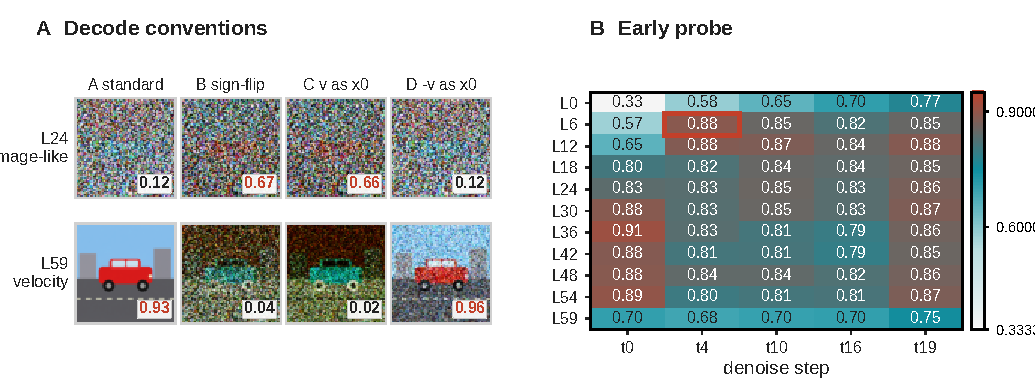
\includegraphics[width=\columnwidth]{figs/fig5_mechanism/fig5_mechanism.pdf}
  \caption{\textbf{Decode convention flips; the probe reads early.}
  \textbf{A}: four \emph{car\_red} decodes reverse convention between L24
  and L59. \textbf{B}: a requested-color basis diagnostic reaches $0.883$
  patch-token accuracy at L6/$t$4 while the frozen head still reads noise
  (chance $0.33$). Patches are not independent experimental units; the
  generation-level fixed-prompt result is $0.667$ over 48 generations.}
  \label{fig:mechanism}
\end{figure}

\paragraph{Prediction generalizes and supports selection.}
Table~\ref{tab:early} summarizes continuous-hue replications and held-out
best-of-five tests. Natural-photo mug and tree edits replicate while the
heterochromatic-eyes task is null ($p{=}0.796$); the independent 40-block
Boogu editor also carries an early hue readout, although its terminal layer
is stronger. Selection succeeds on Boogu and two Qwen target tasks. Actual
interrupted captures plus winner reruns save about 68\% versus full
best-of-five, but only select the closest available candidate.

\begin{table}[t]
\caption{Early prediction and held-out selection. Q/B denote Qwen/Boogu;
parentheses give chance or random-selection baselines.}
\label{tab:early}
\centering
\footnotesize
\setlength{\tabcolsep}{2.1pt}
\begin{tabular}{@{}lllll@{}}
\toprule
Setting & Readout & Metric & Result & Evidence \\
\midrule
Car fixed & Q L6/$t$4 & Bal. acc.$\uparrow$ & .667 (.333) & $p{=}.002$ \\
Car hue & Q L6/$t$2 & MAE$\downarrow$ & $22.3{\to}8.3^\circ$ & $R^2{=}.815$ \\
Tree hue & Q L6 & MAE$\downarrow$ & $55.9{\to}11.4^\circ$ & $p{=}.005$ \\
Mug hue & Q L6 & MAE$\downarrow$ & $17.0{\to}10.7^\circ$ & $p{=}.005$ \\
Boogu hue & B L4/$t$2 & MAE$\downarrow$ & $39.9{\to}6.9^\circ$ & $p{=}.005$ \\
Boogu select & B L4 best-5 & Success$\uparrow$ & 8/12 (20\%) & $p{=}4.1{\times}10^{-5}$ \\
Tree select & Q L6/$t$2 & MAE$\downarrow$ & $95.2{\to}46.5^\circ$ & $p{=}3.7{\times}10^{-7}$ \\
Car select & Q best-5 & MAE$\downarrow$ & $25.7{\to}11.1^\circ$ & $p{=}.0086$ \\
\bottomrule
\end{tabular}
\end{table}

\paragraph{Where the instruction enters.} A complementary text-stream
ablation locates where the prompt is \emph{consumed}: zeroing the model's
text tokens in only the first 11 blocks garbles the whole scene, while
zeroing them after layer 36 barely dents the edit ($P(\text{red}){=}0.993$).
The instruction is fused into the image stream early; for this color edit,
later text tokens are dispensable by layer 36 -- the ``injection'' stage of the circuit in
Figure~\ref{fig:teaser}, whose full text-band table is in the supplement.
Together with the probe, this gives the paper's five-stage picture:
injection ($\le$L36), early outcome prediction, a target-image code, translation
(L52--54), and the output head.
\noindent\textbf{Takeaway.} Time onset is mostly immediate; the frozen depth
lens looks late, but generation-level probes read the realized outcome from L6.

\subsection{The Edit Is Translated Late: Two Codes}\label{sec:translate}

\noindent\textbf{Question.} If probes read the outcome early, what mid-stack
code is converted at L52--54? Three measurements answer this: at an intermediate layer
the frozen head yields a per-token vector $v_\ell$ we normally treat as a
velocity, forming $\hat x_0 = x_t - \sigma_t v_\ell$ (variant A). Decoding
$v_\ell$ instead \emph{directly}, as if it were already a clean latent
(variant C), inverts the story: for \emph{car\_red} at step 4, at L24 the
standard decode A scores $P(\text{red}){=}0.12$ (still wrong-colored)
while the direct decode C already scores $0.66$; at L59 this reverses (A
$=0.93$, C $=0.02$). The mid-stack is not blank -- it encodes the target
content in an \emph{image-like} convention, and a narrow band near the top
reconciles it to the velocity convention the head consumes. (This is a
whole-vector reweighting, not a literal sign flip: essentially no
individual channel of $v_\ell$ has a negative slope against $v_{59}$, mean
$0.003$.)

\paragraph{The conversion location is stable; its width is timestep-dependent.} A dense
every-layer sweep from L44 to L59 (Figure~\ref{fig:boundary}) locates the
A/C crossover precisely: transition midpoint L53.6 at step 16 (width one
layer) and L52.7 at step 4 (width four layers). The midpoints differ by
under one layer, so the boundary's \emph{location} is stable across these
timesteps even though its sharpness is not. Crucially, the
cross-seed probe accuracy is close to \emph{flat} ($0.77$--$0.84$) across
every layer from L44 through L58 and drops only at the terminal layer L59
($0.68$--$0.70$). So the translation that changes what the head can read
(L52--54) and the loss of linear separability (L59) are two \emph{distinct}
events sharing a neighborhood: the target-image code survives the
translation intact and is degraded only by the final, velocity-specific
projection. Coarse family sweeps place measurable style and background
crossovers in the same terminal band; removal and addition remain
inconclusive because their between-variant CLIP margins are too small.

\begin{figure}[t]
  \centering
  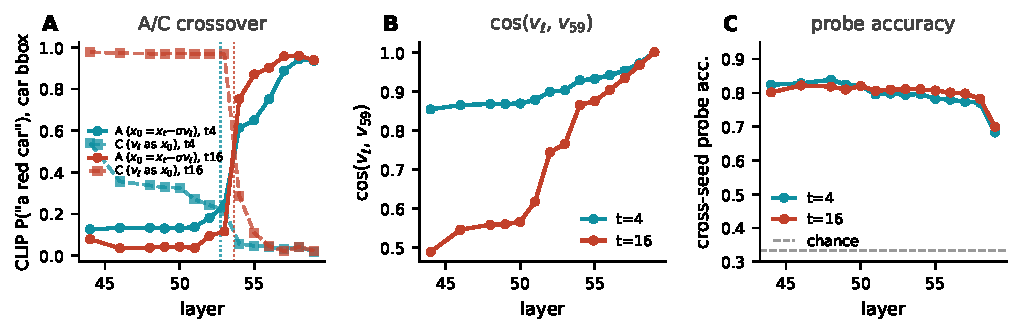
\includegraphics[width=\columnwidth]{figs/fig10_boundary/fig10_boundary.pdf}
  \caption{\textbf{Translation near L52--54.} Dense L44--L59 sweep on
  \emph{car\_red}. \textbf{A--B}: the decode-crossover midpoint changes by
  under one layer between $t{=}4,16$, while transition width changes from
  four layers to one. \textbf{C}: probe accuracy stays flat through L58 and
  drops only at L59.}
  \label{fig:boundary}
\end{figure}

\paragraph{A tuned lens renders the image-like code, layer by layer.} To
test whether the mid-stack code is image-like rather than a probe
artifact, we fit a per-(layer, timestep) tuned lens, as described
above, on exactly three source images -- one each from
\emph{remove}/\emph{background}/\emph{addition} -- and evaluate the entire
\emph{car\_red} source and color family \emph{zero-shot}. Held-out $R^2$
rises with depth from $0.73$--$0.89$ at L6 to
$0.998$ at L59, whose frozen-head decode reproduces the true velocity
bit-for-bit. Every tested depth down to L6 yields a coherent scene, refuting
a pre-registered readability boundary: L52--54 marks the frozen head's
projection, not the representation. At step 0 the pixels are pure noise, yet
Figure~\ref{fig:tunedlens} shows the blue car at L24, orange-red at L36, and
fully red at L52. The dictionaries transfer without retraining to six further
held-out edits; \emph{add\_runner} also reproduces delayed onset internally.

\begin{figure}[t]
  \centering
  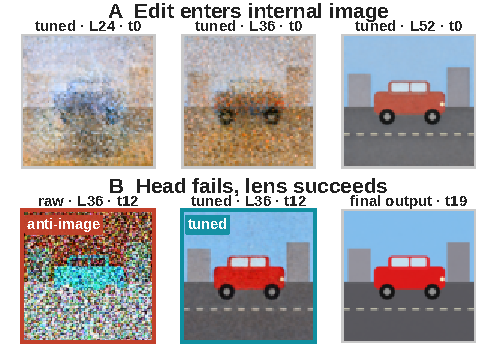
\includegraphics[width=0.98\columnwidth]{figs/fig12_tuned_lens/fig12_tuned_lens.pdf}
  \caption{\textbf{Internal image vs.\ frozen-head ghost.} \textbf{A}: the
  zero-shot tuned lens shows the edit enter a coherent internal image at
  $t{=}0$. \textbf{B}: for the same L36/$t$12 state, the frozen head yields
  an anti-image while the tuned lens recovers the edited scene.}
  \label{fig:tunedlens}
\end{figure}

\paragraph{The anti-image, mechanized.} This also explains a striking
artifact: the mid-stack \emph{frozen}-head decode at later steps is a
color-\emph{inverted} ghost (a cyan car under a red-brown sky) -- the
image-like mid-stack code forced through a head built to consume a
velocity, since $\hat x_0 = x_t - \sigma v$ flips the sign of an
image-like quantity. The tuned lens at the same cell is already coherent.
\noindent\textbf{Takeaway.} Mid-stack states are image-like; the L52--54 band
reconciles them to the velocity convention the head consumes.

\subsection{Transplantable, Writable, and Carrier-Bound}\label{sec:dissoc}

Reading a lens shows only that a representation is \emph{consistent with}
an edit, not what it can install. Whole-token ablation across many layers
drives the edited region off-manifold, so we use it only as a coarse stress
test rather than evidence for fine-grained necessity.

\paragraph{Transplant establishes sufficiency.} Transplanting a
\emph{car\_red} donor's car-region hidden states into a \emph{car\_green}
recipient (which alone scores $P(\text{red}){=}0.011$) flips the output to
red from \emph{any} of four donor bands, including \textbf{L48--59}
($0.940$). The donor representation is therefore sufficient to install
the edit. A content control confirms specificity: splicing the same
donor's \emph{background}-region tokens (right band, wrong content) yields
a garbled ``blue car'' ($0.991$), not red.

\paragraph{Readability does not imply unconstrained writability.} A single stored
\emph{direction} -- the probe's $d_{\text{red}}$, no donor pass -- added to
the recipient's car rows gives a sharp sigmoidal dose-response ($0.024$ at
$\alpha{=}0.5$, $0.977$ at $\alpha{=}1$, saturating to $\alpha{=}8$); a
random direction of equal norm is inert ($0.017$), and the negated
direction overshoots to blue ($0.945$), reproducing the anti-image under
an active intervention. But writability is bounded: at effective doses the
steered region is not a recolored car but a flat red patch that
\emph{replaces} the car's geometry -- the direction installs \emph{which}
hue, not \emph{where to stop}. Supplying that missing ``where'' with the
edited object's own silhouette mask turns every previously-failing dose
into a clean in-place recolor (Figure~\ref{fig:carrier}). And conjuring an
\emph{object} outruns any single direction: the
identity probe direction is inert (the read and write subspaces
differ), while a rank ladder over the donor$-$recipient difference
resolves identity coarse-to-fine -- category at rank 1, a coherent
instance by rank 4, donor-faithful by rank 64 ($2\%$ of the model
dimension). The read and write subspaces differ, and a writable attribute
still requires a spatial carrier.

\begin{figure}[t]
  \centering
  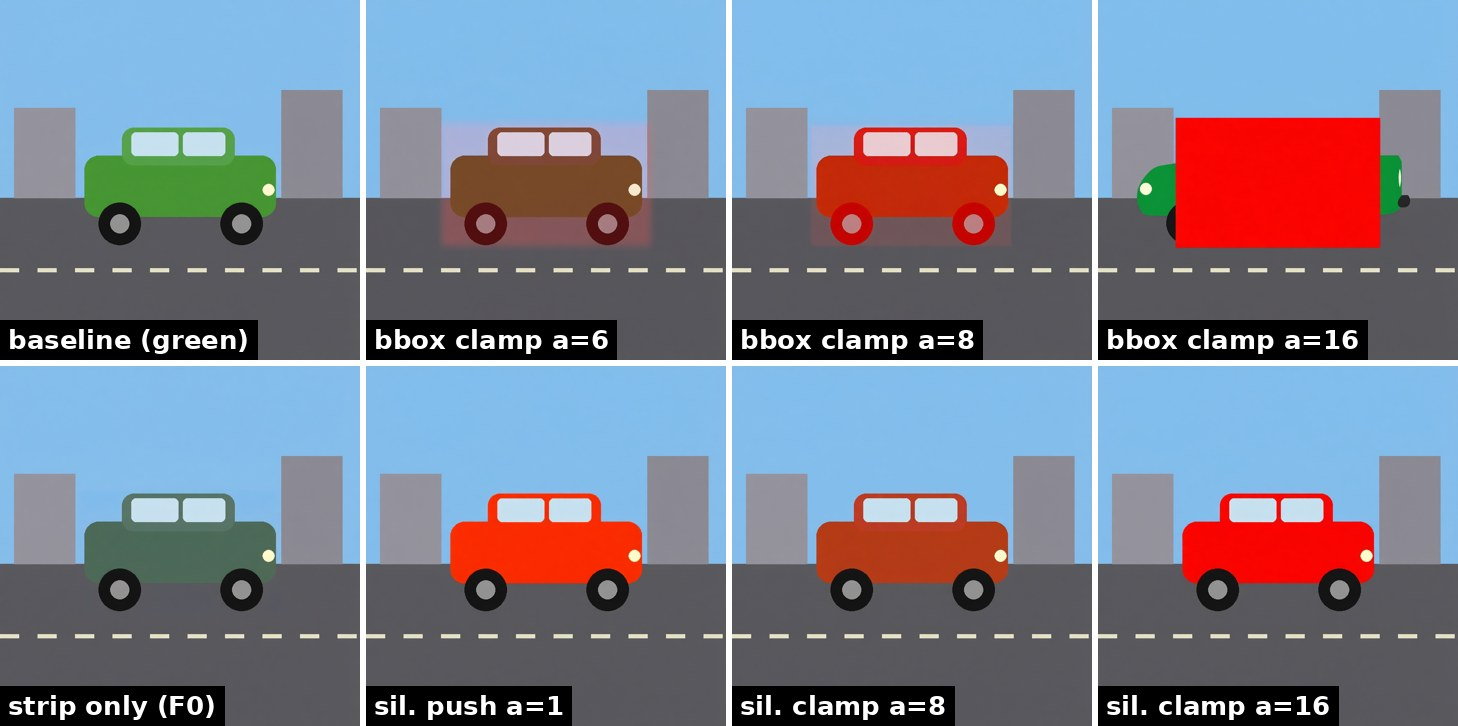
\includegraphics[width=0.48\columnwidth,viewport=0 363 364 726,clip]{figs/i1d_recompose_grid/i1d_recompose_grid.jpg}\hfill
  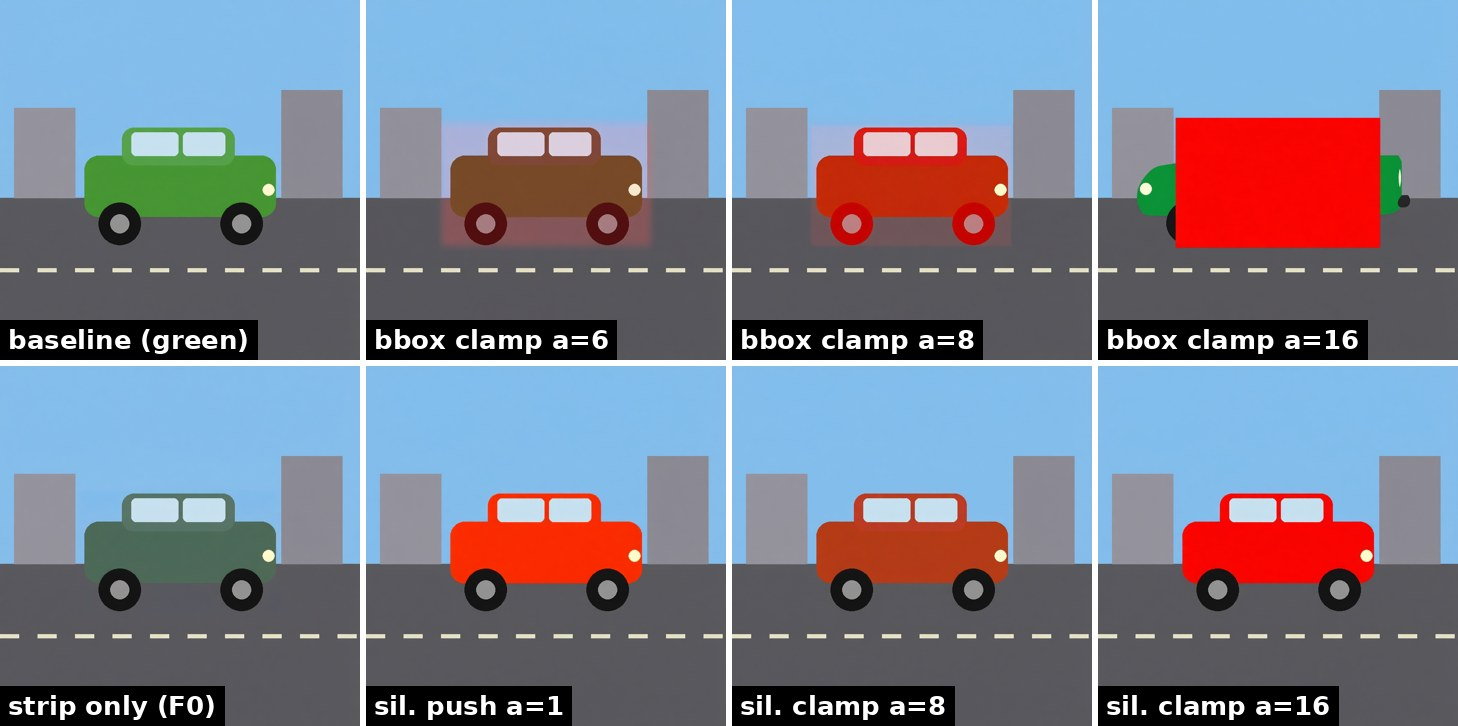
\includegraphics[width=0.48\columnwidth,viewport=1094 363 1458 726,clip]{figs/i1d_recompose_grid/i1d_recompose_grid.jpg}\\[-1pt]
  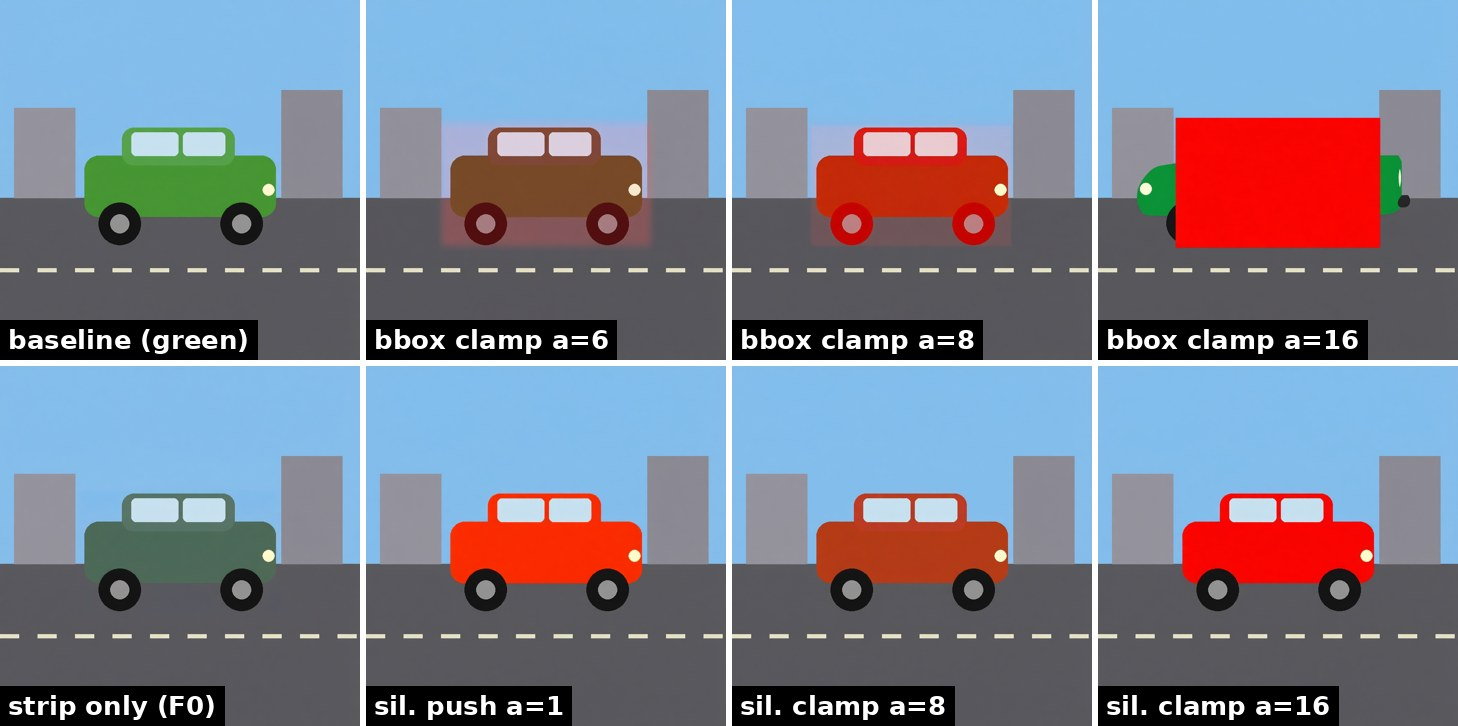
\includegraphics[width=0.48\columnwidth,viewport=729 0 1094 363,clip]{figs/i1d_recompose_grid/i1d_recompose_grid.jpg}\hfill
  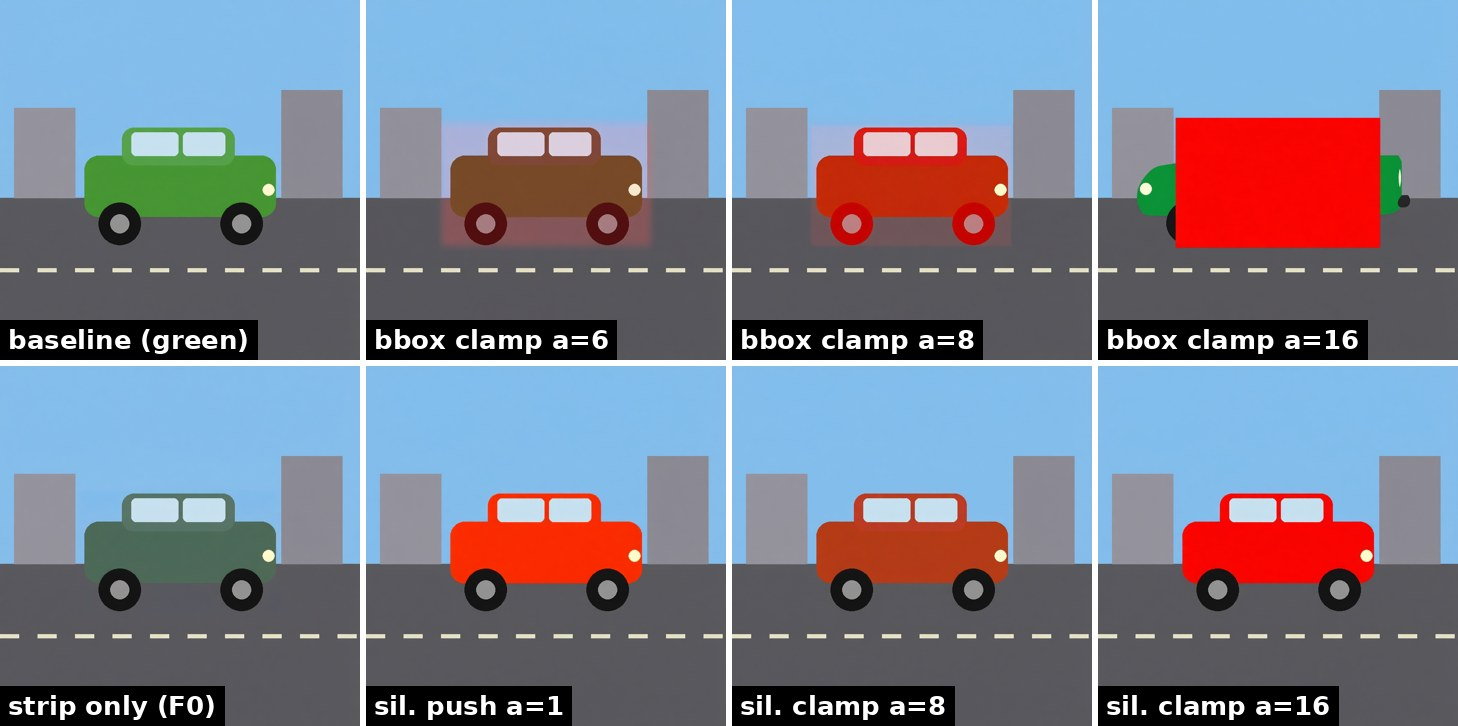
\includegraphics[width=0.48\columnwidth,viewport=1094 0 1458 363,clip]{figs/i1d_recompose_grid/i1d_recompose_grid.jpg}
  \caption{\textbf{A spatial carrier restores clean writability.}
  Steering red inside a bounding box eventually overwrites the car with a
  flat patch (top); the same direction restricted to the car silhouette
  preserves geometry across effective doses (bottom).}
  \label{fig:carrier}
\end{figure}

\paragraph{Rank controls isolate the object write basis.} On one fixed
61-patch lake hull, projecting only the donor--recipient difference's top
singular modes gives a coarse-to-fine identity ladder: rank 1 already recruits
the boat category but produces an incoherent cluster; rank 4 produces one
coherent but wrong instance; rank 16 recovers the donor's wooden material; and
rank 64 ($2\%$ of model width, $89\%$ of difference energy) approaches the
full donor transplant. A same-dimensional random rank-64 basis is inert. Thus
the ladder reflects alignment to a donor-derived write subspace, not merely
intervention rank, and explains why a linearly readable identity probe need not
be directly writable.

\paragraph{Coherent interventions conserve attention routing.} Why does a
full-state transplant preserve the car while direction steering overwrites it?
Following a reference-matched routing audit used for visual-token reduction
~\citep{cho2026restore}, a side recorder recomputes conditional-pass joint attention without changing
the model output, over five seeds, five layers, five steps, three query groups,
and four key groups. Relative to the natural red-edit reference, the
content-matched transplant changes routing by only $0.0031$ total variation and
preserves a coherent car in 5/5 seeds (Table~\ref{tab:routing}). An equal-size
background transplant is as distorted as destructive zero/mean overwrite and
fails in 5/5. Red-direction steering writes red in 5/5 but also has high routing
distortion and produces the flat patch in Figure~\ref{fig:carrier}. Across
seeds, the most distorted coherent condition remains below the least distorted
incoherent one in 5/5 (mean gap $0.0430$, exact one-sided sign-flip
$p{=}0.031$). This supports routing conservation as an explanation for the
tested coherent transplant; it is not a necessity or architecture-general
claim.

\begin{table}[t]
\caption{Attention-routing audit on the car intervention. TV is distortion
from the natural red-edit reference ($\downarrow$); coherence is a blinded
image-level verdict over five seeds.}
\label{tab:routing}
\centering
\footnotesize
\setlength{\tabcolsep}{4pt}
\begin{tabular}{@{}lcc@{}}
\toprule
Intervention & Routing TV $\downarrow$ & Coherent \\
\midrule
Car-state transplant & .0031 & 5/5 \\
Red-direction steer & .0546 & 0/5 \\
Zero overwrite & .0620 & 0/5 \\
Mean overwrite & .0668 & 0/5 \\
Background transplant & .0677 & 0/5 \\
\bottomrule
\end{tabular}
\end{table}

\subsection{A Preview Lever: The Differential Lens at 15\% NFE}\label{sec:difflens}

The differential lens (\emph{Proposed Method}) isolates the internal
edit plan from the reconstruction. It first settles a caveat left open
above: token-level $R^2$ \emph{inside} the edit region is
$0.88$--$0.97$, matching the full-image value, so the tuned
dictionaries carry the edit-specific signal itself, not incidental
scene detail.

\paragraph{Content is early; separation is gradual.} A pre-registered
prediction that $D$ would already localize tightly at every step is
refuted, informatively. The edit \emph{content} is present at step 0 (the
tuned lens already shows red eyes, a black trunk), but the
\emph{differential} at step 0 is a diffuse whole-frame field -- the edit
prompt perturbs the entire velocity relative to the no-op, not just the
edited region -- and condenses onto the edit's footprint only gradually
(localization of $D$'s top mass at L52 climbs monotonically across steps,
e.g.\ $0.21{\to}0.47{\to}0.67{\to}0.83$ for a cat's-eyes recolor).
\emph{Present} (content in the internal image) and \emph{separated}
(the differential has found where it lives) are different quantities.
The no-op control also caught one flat-art scene that \emph{cannot}
``do nothing'' (it renders a transparency checkerboard, and is
discarded), motivating the control-fidelity gate applied before any
differential number is trusted.

\paragraph{A preview lever.} Because the differential carries the edit's
footprint, we ask whether it does so early enough to be useful. At step 2
-- the third of 20, $\approx$15\% of the forward passes -- across a
10-case, five-family battery of natural photographs (all passing the
control-fidelity gate, $r\in[0.86,0.99]$), the median IoU between
$D_{\text{L52},t2}$'s top mass and a final-output difference mask is $0.33$,
$6.6\times$ chance, and all 10 cases sharpen from step 0 to step 2
(Figure~\ref{fig:preview}): an object slated for removal lights up as a
ghost, a keep-vs-replace background segmentation emerges unsupervised, and
a tiny recolor glows at its exact site. Because the no-op control is
\emph{independent of the edit prompt}, it is computed once per source
image and cached; previewing a \emph{candidate} edit then costs three
forward passes plus one frozen-dictionary decode, not a full 20-step run
-- a training-free way to triage many prompts against one image before
running any to completion.

\begin{figure}[t]
  \centering
  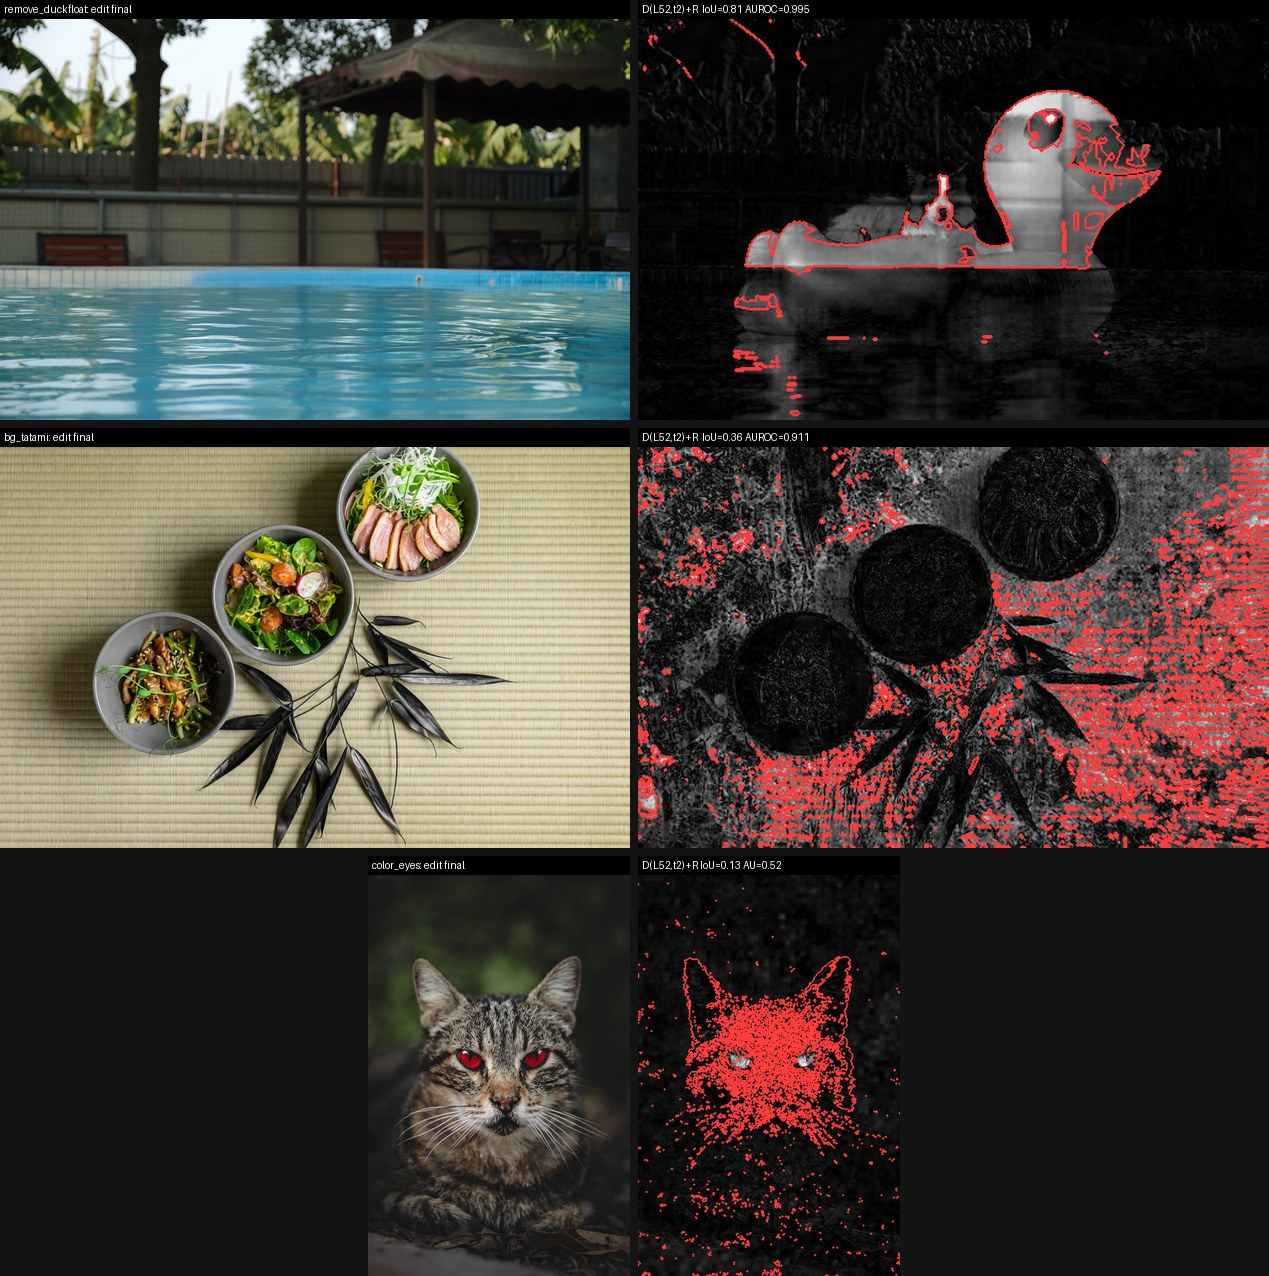
\includegraphics[width=0.84\columnwidth]{figs/fig15_preview_lever/fig15_preview_lever.jpg}
  \caption{\textbf{Differential preview at 15\% NFE.} Final/preview pairs for
  removal, background replacement, and recolor after three of twenty steps;
  red contours mark the final difference mask.}
  \label{fig:preview}
\end{figure}

\subsection{Generalization Across Checkpoints}\label{sec:generalize}

Most mechanistic findings so far concern one model lineage. We re-ran the depth-lens
crossover and cross-seed probe on the two
further checkpoints from \emph{Setup} (FireRed-Image-Edit-1.1 and
Rapid-AIO). \textbf{The translation boundary and explicit-prompt early
readability replicate} (Table~\ref{tab:generalize}). FireRed has the same
flat-then-dip probe shape, and Rapid-AIO preserves the boundary under a
four-step schedule. The readable direction also transfers between Qwen and
FireRed, rather than merely recurring at the same layer index. The full tuned
lens ports to FireRed as well (deep-layer $R^2$ $0.97$--$0.999$; anti-image
reproduced).

\paragraph{The readout basis transfers, not only the boundary.} A three-rung
ladder decodes FireRed with the Qwen translator dictionary frozen (L0), with
only FireRed calibration substituted (L1), or with a fully native refit (L2).
Across a six-case held-out battery spanning five edit families, all 108 deep
cells (six cases $\times$ L52/56/59 $\times$ six steps) order
$\mathrm{L0}<\mathrm{L1}<\mathrm{L2}$; recalibration recovers a median $89\%$
of the frozen-to-native
gap, while the fully frozen dictionary never falls below $R^2{=}0.86$. Even
\emph{style\_ink}, a family absent from translator fitting, has a frozen floor
of $0.885$. Thus the deep readout basis is reusable within this model lineage,
although its calibration remains checkpoint-specific; this does not test an
architecturally unrelated DiT.

\paragraph{The differential law and preview lever transfer.} On two held-out
FireRed photos that pass the unchanged-control gate ($r{=}0.933/0.990$), L52
localization rises with denoising for both tree recolor ($0.90{\to}0.97$) and
runner addition ($0.29{\to}0.84$). Their $t{=}2$ preview IoUs are $0.676$ and
$0.217$, above the registered $0.15$ threshold and $0.05$ chance, and both
improve over $t{=}0$ ($0.610/0.142$). Early content, gradual separation, and
the three-step preview therefore reproduce on this fine-tuned checkpoint.

\paragraph{Noise level, not schedule index, keys the dictionary.} At the Rapid
step where fractional-position and $\sigma$ matching differ, $\sigma$ matching
wins all six deep cells (median $+0.055$ $R^2$). Within $\sigma$ coverage, the
frozen Qwen readout reaches $R^2{=}0.927$--$0.995$ and ties a Rapid-native refit
in 13/24 cells; only the uncovered terminal $\sigma{=}0.02$ fails, and a matched
entry recovers it. Thus the dictionary is keyed to noise level, not sampler
position.

\begin{table}[t]
\caption{Cross-checkpoint boundary/probe transfer
(Qwen$\leftrightarrow$FireRed); L12/$t$4 direction cosine is .833.}
\label{tab:generalize}
\centering
\scriptsize
\setlength{\tabcolsep}{3pt}
\begin{tabular}{@{}lccc@{}}
\toprule
Checkpoint & A/C band & Probe: early $\to$ L59 & Transfer \\
\midrule
Qwen & L52--54 & .883 @ L6/$t$4 $\to$ .68--.70 & source \\
FireRed & L53--56 & .852 @ L6/$t$4 $\to$ .69--.70 & .840/.917 \\
Rapid-AIO & L52--54 & -- & -- \\
\bottomrule
\end{tabular}
\end{table}

\subsection{A Training-Free Lever: Truncating Classifier-Free Guidance}\label{sec:lever}

Running the unconditional pass only for the first two of 20 steps leaves all
tested families intact at a \textbf{45\% reduction in forward passes}; a
20-case battery confirms it (mean $1.77\times$ speedup). With no CFG, recolor,
removal, and addition still land, but background replacement composites around
un-erased source structure ($P(\text{beach}){=}0.45$ vs.\ ${\ge}0.996$),
consistent with a non-redundant role in scope resolution. A four-step distilled
checkpoint also lands 20/20 cases ($7.7\times$ faster), preserving the exposed
structure while compressing the sampling trajectory.

\subsection{Limitations}\label{sec:limits}

Translation/intervention evidence uses Qwen plus two same-lineage checkpoints;
Boogu supports only outcome prediction/selection. The fixed-prompt probe has
one synthetic source and two natural-image replications; one eye case is
unsuitable. Selection has 12 groups per task and cannot create absent targets.
One-way L6 hue transfer (mug$\to$tree $p{=}0.002$; reverse $p{=}0.968$)
precludes an object-invariant subspace. Because CLIP can prefer a flat patch to
a true recolor, quantitative claims carry pre-registered visual verdicts. The
dense boundary and carrier study center on the flat-art car; its silhouette
comes from a source--edit difference, not automatic segmentation. The fixed
top-10\% preview mask can over-expand tiny edits, so IoU is a localization
diagnostic, not segmentation ground truth. We claim tested predictability,
transplant sufficiency, and carrier-bounded writability, not commitment or
necessity.
% END expanded input: aaai_draft/20_experiments

% BEGIN expanded input: aaai_draft/60_conclusion
\section{Conclusion}\label{sec:conclusion}

Outcomes are predictable early; Qwen-lineage image codes translate to velocity
late. The lenses separate readability, sufficiency, and carrier-bounded
writability without claiming commitment, necessity, or universality.
% END expanded input: aaai_draft/60_conclusion

\clearpage
\bibliography{references}

\end{document}
